\chapter{Boson simulations}
\label{ch:Simulations}

\section{Introduction}
\label{sec:SimIntro}
This formed the bulk of the experimental work in my PhD. Roughly speaking, we
take a hamiltonian, \(\mat{H}\) and exponentiate it to get a load of unitaries
(\(\mat{U}=e^{-i\mat{H}t}\)) at a series of timesteps. Using a decomposition
similar to the one in \cite{reck} we can implement these on a single
circuit.

Two physical implementations: bulk optics and integrated optics. I was
responsible for the calibration of the bulk circuit (crapusoids), writing the
control code, and taking a large portion of the data. I trained DTC student
Chris Sparrow in the operation of the experiment.

\begin{figure}
  \centering
  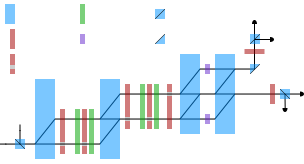
\includegraphics{figures/circuit.pdf}
  \caption[A schematic of the bulk optics circuit used for simulations.]
  {A schematic of the bulk optics circuit. Two photons are injected at
  the left of the circuit in orthogonal polarisations (\(\ket{H}\) indicates
  horizontal and \(\ket{V}\) indicates vertical), using an in-fibre polarising
  beamsplitter (PBS) to combine the two photons into a single path. The circuit
  operates in a combined path/polarisation encoding, where polarising beam
  displacers (PBD) are used to convert between the two. Operations are performed
  with fixed quarter waveplates (QWP) and polarisation flips (X), and variable
  angle half waveplates (HWP). After the operations are complete,
  polarisation-sensitive detection is performed using further PBS elements and
  single photon avalanche diodes. We label the detectors A through D.}
  \label{fig:circuit}
\end{figure}

\section{Quantized vibrational states}
\label{sec:Phonons}
More background: introduce the idea of quantized vibrational states and present
the data for the 4-atom ring. I took the data, and did some of the analysis.

\section{Molecular vibrations}
\label{sec:Molecules}
Simulating phonons in the harmonic limit corresponds to vibrations of molecules.

\section{PT-symmetric systems}
\label{sec:PT}
\subsection{Introduction}
In a seminal lecture \cite{qsim-feynman}, Feynman proposed that the
fundamentally quantum nature of microscopic systems will enable an exact
simulation of nature using quantum computers. Since then, tremendous progress
has been made towards the development of such computers that, at their heart,
are quantum systems \cite{qcomp-review}. On a broader scale, the
development of tunable, controlled physical systems that simulate, on a quantum
level, the phenomena of interest has been vigorously pursued over the past
decade. Optical lattices have been used to simulate Mott-insulator transitions
\cite{jordens-nature-455-204}, synthetic magnetic fields
\cite{lin-nature-462-628} and bound states in a repulsive potential
\cite{winkler-nature-441-853}. Evanescently coupled waveguides
\cite{garanovich-waveguides-2012} have been used to simulate quantum
correlations \cite{walks-peruzzo}, disorder effects
\cite{crespi-nphoton-7-322} and tunable quantum statistics
\cite{matthews-scirep-3-1539}, as well as exotic states such as Floquet
topological insulators \cite{rechtsman-nature-496-196,
khanikaev-natmater-12-233} and quantized Landau levels
\cite{rechtsman-nphoton-7-153}.

Concurrently, the groundbreaking work by Knill Laflamme and Milburn
\cite{klm} has shown that an arbitrary quantum simulation can be
implemented efficiently using linear optical elements along with single photon
sources and detectors \cite{kok-revmodphys-79-135}, and significant advances
have been made in increasing the efficiency and reducing the ancillary resources
required for such an implementation \cite{review-obrien,
obrien-natphoton-3-687}. In all their manifestations, the goal of quantum
simulators has been to simulate closed quantum systems with a unitary time
evolution \cite{cirac-natphys-8-264}: the effective Hamiltonian that describes
such systems is always Hermitian.

On a disparate front, non-Hermitian Hamiltonians, \(\mat{H}_{\pt}\), that are
invariant under the combined parity \((\op{P})\) and time-reversal
\((\op{T})\) operations have been theoretically explored for more than a
decade \cite{bender98, levai-jphysa-33-7165, bender07}. Although not Hermitian,
such \(\pt\)-symmetric
Hamiltonians have a purely real spectrum that changes into complex-conjugate
eigenvalues as the non-Hermiticity is increased. When the spectrum of
\(\mat{H}_{\pt}\) is purely real, its non-orthogonal eigenvectors are
simultaneous eigenvectors of the \(\pt\) operation. However, when the spectrum
has complex conjugate eigenvalues, due to the anti-linear nature of the operator
\(\op{T}\), the eigenvectors are not \(\pt\) symmetric. This transition from
real to complex spectrum is called \(\pt\) symmetry breaking. 

It has been established that \(\pt\) symmetric theory is unlikely to be a
complete alternative to quantum mechanics, either reducing to the same thing
\cite{mostafazadeh-jmathphys-43-205} or producing non-physical results such as
violation of the no-signaling principle of relativity \cite{lee-prl-112-130404}.
However, it has recently become clear that it is far from being just a
mathematical curiosity: \(\pt\)-symmetric Hamiltonians model open
systems---classical or quantum---with balanced, spatially separated loss and
gain. They have been used to theoretically investigate vortex hopping in
superconductors \cite{naomichi-physrevlett-77-570},
statistical mechanics of Coulomb gases \cite{gulden-jetp-117-517} and
Non-equilibrium superconductivity \cite{rubinstein-physrevlett-99-167003,
serbyn-physrevb-87-020501}. During the past three years, the \(\pt\)
symmetry breaking has been experimentally investigated in classical systems
including two optical waveguides \cite{pt-ruter}, electrical circuits
\cite{schindler-physreva-84-040101}, mechanical systems
\cite{bender-amjphys-81-173} and discrete fiber networks
\cite{pt-regensburger}.

In this paper, we demonstrate the quantum simulation of non-interacting bosons
evolving under a \(\pt\) symmetric
Hamiltonian. We investigate the single-particle statistics and bosonic
correlations across the \(\pt\) symmetry breaking threshold. Although the time
evolution under \(\mat{H}_{\pt}\) is not unitary, by embedding this open system
into a larger, closed system, we demonstrate a general method for simulating
non-Hermitian Hamiltonians.

\begin{figure*}[t]
  \centering
  \includegraphics[width=\textwidth]{figures/protected/fig1}
  \caption[Schematic of the system and manifold for results]
    {(a) Schematic of the system, showing how the introduction
    of coupling to an environment allows us to model the non-unitary system in
    linear optics. (b) The linear-optical circuit used to perform the
    experiment. Photon pairs from a type-I SPDC source are injected in the left,
    and operations are performed on the polarisation state of the photons using
    bulk-optical components. Half waveplates (HWP) control amplitude splittings,
    while phase shifts are performed with a series of three waveplates (QHQ): a
    half waveplate between two quarter waveplates oriented with the optic axis
    at 45 degrees. Polarisation is flipped from horizontal to vertical using
    fixed blocks (X), and conversion between path and polarisation is performed
    with either beam displacers (BD) or polarising beamsplitters (PBS).
    (c) Time evolution of the occupation of the initially occupied
    mode (\(S_1\)) after evolution, for various suttings of the complex on-site
    potential, \(\gamma\) across the \(\pt\) boundary. Coloured lines (red for
    \(\pt\) symmetric, green for \(\pt\) critical and blue for \(\pt\) broken)
    show cross-subsections where experimental data are taken. (Note the logarithmic
    scale used in the \(z\) axis, since occupation in the \(\pt\)-broken region
    increases exponentially. (d) The same time evolution as (c), but showing the
    measured output power before any scaling. Coloured lines show the
    cross-subsections as in (c); the points show the experimental data.}
  \label{fig:manifold}
\end{figure*}

\subsection{Theory}
\subsubsection{Two-site \(\pt\)-symmetric model}
Let us consider a 2-site Hamiltonian with a tunneling \(J > 0\) between the two
sites and a \(\pt\)-symmetric potential \(\pm i \gamma\) on the two sites, \(
\mat{H} = -J \sigma_x -i \gamma \sigma_z\). The eigenvalues of this matrix are
\( \epsilon = \pm \sqrt{J^{2} - \gamma^{2}} \) which are real for \( J \geq
\gamma \), although the eigenvectors are not orthogonal to each other.

First, let us assume that the non-Hermitian term is small, i.e. \( \gamma \leq
J \) and \( \epsilon \) is real. In this case, we get the following
(non-unitary) time-evolution operator with \( \alpha = \epsilon \frac{t}{\hbar}
\)
\begin{equation}
  \mat{G}_{\leq} \of{t} = \begin{pmatrix}
    \cos \alpha - \frac{\gamma}{\epsilon} \sin \alpha &
    i \frac{J}{\epsilon} \sin \alpha \\
    i \frac{J}{\epsilon} \sin \alpha &
    \cos \alpha + \frac{\gamma}{\epsilon} \sin \alpha
  \end{pmatrix}
\end{equation}

In the limit where \( \gamma \rightarrow J_{-} \), \( \epsilon \rightarrow 0 \)
and \( \frac{1}{\epsilon} \sin \alpha \rightarrow \frac{t}{\hbar} \), thus at
the \(\pt\) phase boundary the time evolution operator becomes linear in time
instead of sinusoidal:
\begin{equation}
  \mat{G}_{\leq,-} = \begin{pmatrix}
    1-J\frac{t}{\hbar} & i J\frac{t}{\hbar} \\
    i J\frac{t}{\hbar} & 1+J\frac{t}{\hbar}
  \end{pmatrix}
\end{equation}
This also follows from the fact that \( \mat{H}^{2} = 0\) when \(J = \gamma\),
thus \( \mat{G}_{\leq} \of{t} \) truncates to the first two terms.

If we allow a large non-Hermitian term, \( \gamma \geq J \), then the
eigenvalues are purely imaginary, \( \epsilon = \pm i \sqrt{ \gamma^{2} - J^{2}
} = i \Gamma \). The corresponding eigenvectors are still not orthogonal. In
this case, the time evolution operator (with \( \beta = \Gamma \frac{t}{\hbar}
\)) is
\begin{equation}
  \mat{G}_{\geq} \of{t} = \begin{pmatrix}
    \cosh \beta - \frac{\gamma}{\Gamma} \sinh \beta &
    i \frac{J}{\Gamma} \sinh \beta \\
    i \frac{J}{\Gamma} \sinh \beta &
    \cosh \beta + \frac{\gamma}{\Gamma} \sinh \beta
  \end{pmatrix}
\end{equation}
In the limit where \( \gamma \rightarrow J_{+} \), \( \Gamma \rightarrow 0 \)
and \( \frac{1}{\Gamma} \sinh \beta \rightarrow \frac{t}{\hbar} \) thus at the
\(\pt\) phase boundary, we get a continuous time evolution operator,
\begin{equation}
  \left. \mat{G}_{\leq} \of{t} \right|_{\gamma \rightarrow J_{-}} = \left.
    \mat{G}_{\geq} \of{t} \right|_{\gamma \rightarrow J_{+}}
\end{equation}

The behaviour of this \(\pt\)-symmetric system can be understood by looking at
the occupation of (system or environment) modes when a particle initially in the
system is evolved under the non-Hermitian \(\mat{H}\). This will be a function
of the ratio \(\gamma/J\) as well as the time. In figure~\ref{fig:manifold} we
illustrate this by setting \(J=1\) and showing the occupation of one of the
system modes as a function of time for a range of values of \(\gamma\). The
transition from \(\pt\) symmetric to \(\pt\) broken can be seen, and the
occupations are continuous over the boundary. Also shown are cross-subsections
where experimental data are taken (see figure~\ref{fig:results} for full
experimental data).

\subsubsection{Unitary Dilation}
The simulation technique that we use requires that we embed the non-unitary
time-evolution operator into a larger, unitary operator. This can be done for
any matrix by doubling the dimension; that is, any \(n \by n\) matrix can be
embedded as an \(n \by n\) submatrix of a \(2n \by 2n\) unitary matrix. In order
to perform this embedding for a non-unitary matrix \(\mat{G}\), we must first
rescale it so that the operator norm is less than or equal to 1. A suitable
definition of operator norm in this case is \(\abs{\mat{G}} = \sqrt{\abs{e_{
\text{max}}}}\), where \(e_{\text{max}}\) is the largest eigenvalue of 
\(\mat{GG^{\dagger}}\) \cite{dilation}. The scaled matrix is then
\begin{equation}
  G_{s} = \frac{G}{\sqrt{\abs{e_{\text{max}}}}}
\end{equation}
and the unitary dilation can be expressed as follows:
\begin{equation}
  U = \begin{pmatrix}
    \mat{G}_{s} & \mat{D}\of{\mat{G}_{s}} \\
    \mat{D}\of{\mat{G}_{s}^{\dagger}} & -\mat{G}_{s}^{\dagger} \end{pmatrix}
\end{equation}
where \(\mat{D}\of{\mat{G}_{s}} = \left( \identity - \mat{G}_{s}\mat{G}_{s}^{
\dagger} \right)^{\half}
\) is the \emph{defect matrix} of \(\mat{G}_{s}\).

It can be verified by explicit calculation that \(\mat{U}\) is unitary.
Since \(\mat{G}_{s}\mat{G}_{s}^{\dagger}\) is always Hermitian, it always has
real eigenvalues and thus the defect matrix is well defined.

Physically, the interpretation of this unitary matrix corresponds to doubling
the number of available modes by introducing an \emph{enviroment} space, of
equal dimension to the \emph{system}. The rationalisation for this increase in
size being sufficient is that each system mode needs only one loss/gain channel
to realise arbitrary dynamics: adding more does not provide any additional
freedom.

The top left corner contains the matrix
\(\mat{G}_{s}\), which describes motion within the system and the bottom right
corner (\(-\mat{G}_{s}^{\dagger}\)) describes motion within the environment.
Since \(\mat{G}_{s}=\exp \of{-i\mat{H}t}\), the evolution of the environment,
\(\mat{-G}_{s}^{\dagger}=-\exp \of{i\mat{H}t}\), or the time-reversal of the
system's evolution (with a constant phase). The cross terms, \(\mat{D}
\of{\mat{G}_{s}}\) and \(\mat{D} \of{\mat{G}_{s}^{
\dagger}} \), describe the coupling between the system and environment. If
\(\mat{G}_{s}\) is already unitary, this coupling disappears, as expected:
unitary evolution applies to a closed system.

A consequence of this simulation method is that there is no effective
Hamiltonian that models the evolution of the closed system, i.e. no matrix
\(\mat{H}_{\eff}\) can satisfy
\begin{equation}
  U\of{t} = e^{-i\mat{H}_{\eff}t}
\end{equation}
for all times \(t\). This is evident when considering the initial time \(t=0\).
We would require
\begin{equation}
  \mat{U}\of{0} = \begin{pmatrix}
    \identity & 0 \\
    0 & -\identity
  \end{pmatrix}
\end{equation}
which cannot be achieved for any effective Hamiltonian. This observation implies
that the environment modes introduced for the simulation do not really
correspond to a real physical system; rather they are just a convenient way of
keeping track of gain and loss.

\begin{figure*}[t]
  \centering
  \includegraphics[width=\textwidth]{figures/protected/results}
  \caption[Results of simulation]
    {Results of our experimental simulation. The top row (a-c) shows
    single photon data. The photon is initially injected in the system mode
    \(S_1\); probability of detection in each of the four modes \(\left\{S_1,
    S_2, E_1, E2\right\}\) after the evolution is shown. (a) is in the
    \(\pt\)-symmetric region (\(\gamma=0.95\)), where we observe periodic
    behaviour. (b) is on the \(\pt\) phase boundary (\(\gamma=1\)) and (c) is
    in the \(\pt\) broken region (\(\gamma=1.05\)). In both of these cases,
    the detection probabilities in our
    experiment tend towards a constant value, with any evolution after this
    point being purely due to the scale factor. The bottom row (d-f) shows
    two-particle data, where the particles are initially injected in the two
    system modes, \(S_1\) and \(S_2\). We show the detection probabilities for
    pairs where one photon is still in mode \(S_1\), and the other photon is in
    a different mode. (d) is in the \(\pt\)-symmetric region (\(\gamma=0.95\)),
    and again exhibits periodic behaviour. (e) is on the \(\pt\) phase boundary
    (\(\gamma=1\)) and (f) is in the \(\pt\)-broken region (\(\gamma=1.05\)). In
    all cases, the scale factor (black dashed line; on a different axis), has
    been separated out from the experimental observations, which reflect
    detection probabilities, rather than mode occupation.}
  \label{fig:results}
\end{figure*}

\subsection{Experiment}
\subsubsection{Our Simulation}
For our simulation we use a reconfigurable, four-mode photonic circuit in bulk
optics, shown in figure~\ref{fig:manifold}(b). We map two of these optical modes
to the system and two to the environment, so the transformation performed by the
circuit is guaranteed to be unitary. By looking at detection events on only the
system modes, \(S_1\) and \(S_2\) we can observe (a scaled version of) the
evolution of the \(\pt\)-symmetric system, or by considering detection events on
any other modes, we can study the interaction between the system and the
environment. Note that when post-selecting on the system modes, there is a
non-unit probability of a detection event. In light of this, we could not
simulate the super-luminal signalling described in \cite{lee-prl-112-130404}.

The reconfigurability of our circuit is obtained by joint path/polarisation
operations. We can control the amplitudes at the output with half waveplates
(HWPs), and the phases with a series of three waveplates (QHQ): a half waveplate
between two quarter waveplates with the optic axis orientated at 45 degrees.
We use beam displacers (BDs) to convert between path and polarisation and
implement very stable Jamin-Lebedeff interferometers, while
polarisation-sensitive detection is achieved with in-fibre polarising
beamsplitters (PBS) and single-photon avalanche diodes (SPADs).

\subsubsection{Results}
The graphs in figure~\ref{fig:results} show the evolution of the 2-site system
at 3 points in the parameter space: \(\pt\)-symmetric, \(\gamma=0.95\) (a,d);
\(\pt\)-critical, \(\gamma=1.0\) (b,e) and \(\pt\)-broken, \(\gamma=1.05\)
(c,f). The scale factor (i.e. operator norm of the non-unitary matrix) has been
seperated from the experimental data for clarity. Consequently, the occupation
probabilities are always bounded between zero and one, and reflect the
probabilities of detecting photons in the relevant optical modes. On the other
hand, the scale factor is unbounded, and this is the origin of the quadratic or
exponential growth in the critical and \(\pt\) broken regions.

The top row (a-c) shows single-photon data, where the photon is injected into
system mode \(S_1\). Occupation probabilities for all output modes are shown.
The bottom row shows coincidental detections, where the photons are injected
into the two system modes, \(S_1\) and \(S_2\). We show occupation probabilities
for one photon in system mode \(S_1\) and the other photon in a different mode.
In both the \(\pt\)-critical and \(\pt\)-broken regions, the coincidental
detections between system and environment have very low probability.

Throughout all graphs, points represent experimental data (error bars due to
Poissonian noise are too small to see at this scale) and lines represent
theoretical expectations. The dashed black line (not on the same scale) is the
scale factor, and is unbounded.

To evaluate the fidelity of our simulations, we look at two measures. The first
is a trace distance between the unitary matrix that we intended to implement,
and the matrix that we in fact did implement, according to the data we collect
\todo{cite SST}. If the desired unitary is \(\mat{U}\) and the measured unitary
is \(\mat{U^{\prime}}\), the trace distance, \(F\) is defined by:
\[F=\frac{1}{2}\Tr\of{\mat{U}^{\dagger}{\mat{U}^{\prime}}}\]
The second measure we use compares (normalised) discrete probability
distributions, \(p\) and \(q\). This fidelity is computed as:
\[F=1-\frac{1}{2}\sum_{i}\abs{p_{i}-q_{i}}\]
This can be computed for the single photon data without any normalisation, since
detection probabilities in the four modes \(S_1\),\(S_2\),\(E_1\) and \(E_2\)
must sum to 1. In the case of coincidences, we only measure 6 out of the 10
possible pairings, so we must normalise these to 1 before computing the
fidelity.

In summary, the fidelities obtained are \(0.948 \pm 0.052\) for the trace
distance, \(0.956 \pm 0.020\) for the single photon data shown and \(0.961 \pm
0.014\) for the coincidences. Note that the figure for the coincidences takes
into account the \(S_2 E_1\), \(S_2 E_2\) and \(E_1 E_2\) correlations, which
are not presented here.

We have therefore demonstrated the ability to simulate the evolution of
\(\pt\)-symmetric systems in our 2-site model, across all regions of the phase
space. The cost of our implementation using linear optics and unitary dilation
is a doubling in the number of optical modes required, compared to the dimension
of the system we are simulating. However, with integrated optics
\todo{citations}, a constant-factor increase in number of modes is
straightforward to handle. In addition, our method of simulation allows the
number of particles to be scaled up, to the point where classical simulations
may become intractable.

\subsection{Supplementary information}
\subsubsection{Photon source and detectors}
The type-I spontaneous parametric down-conversion source used a 404nm
continuous-wave laser focused to a 40 \(\mu\)m waist in a \(\text{BiB}_3
\text{O}_6\) (Bismuth Triborate) non-linear crystal to produce pairs of
degenerate photons at 808nm. The photon pairs were filtered with high
transmission interference filters of 3nm spectral width and collected into
polarisation-maintaining optical fibres. Single-photon detection was achieved
using silicon-based avalanche photodiode single-photon counting modules.
Coincidence counting logic used a field-programmable gate array.

\subsubsection{Linear optical realisation of any unitary operator}
Any \(m\)-dimensional unitary transformation \(\mat{U} \of{m}\) can be factored
into \(m^{2}\) independent optical components: \(\frac{1}{2} m \left( m-1
\right) \) beamsplitters and \(\frac{1}{2} m \left( m+1 \right) \) phase shifts,
as shown in \cite{reck}.

\subsubsection{Experimental reconfigurable circuit for 4 modes}
The circuit shown in figure~\ref{fig:manifold}(b) can be used to realise any
unitary operator in 4 modes, down to experimentally undetectable phases on the
input and output modes. This insensitivity to certain phases reduces the number
of parameters that we need to control to 7. All of the tunable parameters are
realised experimentally with half waveplates (HWPs), 5 of which control
amplitude splitting and the remaining 2 control internal phases
(interferometers). The amplitude
splittings can be computed easily and deterministically for any matrix. However
the calculation of the internal phases is complicated by the fact that the
interferometric path difference depends on not just the waveplates
that we use to control the phase, but also on other elements inside the
interferometer. Consequently, we use single-photon data to calibrate the
interferometers for each case on an ad-hoc basis. This does not pose a problem
for scalability, since it can be done using classical (coherent) light or
single-photon input states. The single-photon data presented in
figure~\ref{fig:results} do not rely on this calibration.

\subsubsection{Data acquisition}
For each unitary operator that we implement, we take one- and two-photon data.
The one-photon data presented in this paper is obtained by injecting one photon
into the circuit, with the other photon from the created pair acting as a
herald, and counting coincidental detections between them. This data was taken
with an integration time of 30 seconds for each of the two input modes of the
circuit.
% NOTE: Remember that we take the one-photon data with 4 detectors, so we first
% herald with detector A and measure BCD and then herald with detector D and
% measure ABC.
The two-photon data consists of injecting both photons simultaneously then
delaying one photon from the pair with respect to the other to observe the
quantum to classical transition in photon correlations. This is done for each
pair of different output ports giving a total of six pairwise data sets in our
four-mode case. Two-photon data points were taken every 0.02mm over a range of
0.48mm with 20 seconds integration time.

Finally, we measure the relative detector efficiencies for the circuit. To do
this, we inject unheralded photons from one arm of the source through the input
mode \(S_1\), and direct them to each of the output ports in turn. The ratios of
counts at each of detectors \(S_2\), \(E_1\) and \(E_2\) to the counts at
detector \(S_1\) (after an integration time of 20 seconds and subtracting the
background of dark counts) give us the relevant efficiency data. We use this
measured efficiency data to correct both the one- and two-photon count numbers.
